\documentclass[a4paper]{article}
\usepackage{fullpage}
\usepackage{graphicx}
\usepackage{xcolor}

\usepackage{hyperref}

\usepackage{minted}
\usepackage{natbib}

\CatchFileDef{\myversion}{|echo $VERSION}{}

% Define custom color
\definecolor{CustomBlue}{rgb}{0.25, 0.41, 0.88} % RoyalBlue
% Set up hyperref with the custom citecolor
\hypersetup{
    colorlinks=true,
    citecolor=CustomBlue,
    linkcolor=black, % You can set this to any color you prefer
    urlcolor=blue    % You can set this to any color you prefer
}

% Define colors
\definecolor{background}{RGB}{245,245,244}
\definecolor{string}{RGB}{163,21,21}
\definecolor{keyword}{RGB}{0,0,255}
\definecolor{comment}{RGB}{0,128,0}
\definecolor{identifier}{RGB}{0,0,0}
\definecolor{bashkeyword}{RGB}{0,0,128}

% Minted settings
\setminted{
    bgcolor=background,
    fontsize=\footnotesize,
    linenos,
    breaklines,
    frame=single,
    framesep=2mm,
    tabsize=2
}

\begin{document}

\title{Template Repository for Articles\\ \small\tt Version \myversion}
\author{Christophe Prud'homme\thanks{Cemosis, IRMA UMR 7501, Université de Strasbourg, CNRS, France, \tt \href{mailto:christophe.prudhomme@cemosis.fr}{christophe.prudhomme@cemosis.fr}}}
\maketitle
\tableofcontents

\section{Introduction}
\label{sec:introduction}

Writing scientific articles using LaTeX offers numerous advantages, including precise typesetting, seamless integration of references, and robust version control. 
This template repository demonstrates best practices for organizing LaTeX projects, utilizing GitHub Actions for automated document compilation, managing bibliographies with Zotero, and optimizing image handling. 
By following this template, researchers can enhance their workflow efficiency and ensure consistent document formatting across platforms like Overleaf and local LaTeX installations.
The releases assets produced by the GitHub Actions allows to upload the article to HAL, arXiv, Zenodo, etc.

\section{Image Naming Convention}

To ensure compatibility with platforms like HAL, arXiv, and Overleaf, name your images with the \texttt{img-*} prefix and store them in the same directory as the \texttt{.tex} file. 
This makes it easier to manage and upload your images along with your LaTeX document.

\textbf{Example}:
\begin{itemize}
    \item \texttt{img-figure1.pdf}
    \item \texttt{img-figure2.png}
    \item \texttt{img-figure3.jpg}
\end{itemize}

\section{Using References from Zotero via Overleaf}

To manage your references with Zotero and integrate them seamlessly into Overleaf, follow these steps:

\subsection{Export Zotero Library to BibTeX}
\begin{enumerate}
    \item Open Zotero and select the references you want to export.
    \item Go to \texttt{File > Export Library}.
    \item Choose \texttt{BibTeX} as the format and save the file (e.g., \texttt{references.bib}).
\end{enumerate}

\subsection{Upload BibTeX File to Overleaf}
\begin{enumerate}
    \item Open your project in Overleaf.
    \item Click on the \texttt{Upload} button (top-left corner) and upload your \texttt{references.bib} file.
\end{enumerate}

\subsection{Include the Bibliography in Your LaTeX Document}

Add the following lines to your \texttt{.tex} file to include the bibliography:

\begin{minted}[bgcolor=background]{latex}
\documentclass{article}
\usepackage{graphicx}
\usepackage{natbib}
\begin{document}

% Your content here

\bibliographystyle{plainnat}
\bibliography{references}

\end{document}
\end{minted}

\subsection{Cite References in Your LaTeX Document}

Use the \mintinline{latex}{\cite} command to cite references within your document. For example:

\begin{minted}[bgcolor=background]{latex}
As shown by \citet{AuthorYear}, this method is effective.
\end{minted}

\section{GitHub Action Workflow for LaTeX Compilation}

The template article repository workflow uses \cite{cheng_xu_xu-chenglatex-action_2024} \mintinline{bash}{xu-cheng/latex-action} to build the latex document.

The GitHub Action workflow:
\begin{itemize}
    \item Compiles the LaTeX document using \mintinline{bash}{xu-cheng/latex-action}
    \item Uploads the resulting PDF
    \item Creates a release with the PDF as an asset when a new tag is pushed of the type \texttt{v*}, e.g., \texttt{v1.0.0} or a pre-release \texttt{v1.0.0-preview.1}
\end{itemize}

To create a git tag, do the following:

\begin{minted}[bgcolor=background]{bash}
git tag -a v1.0.0 -m "Version 1.0.0"
git push origin v1.0.0
\end{minted}

\section{Steps to Use the Template Repository}

\subsection{Create a New Repository}
Use the git template repository feature to create a new repository based on this template.

\begin{figure}[h!]
\centering
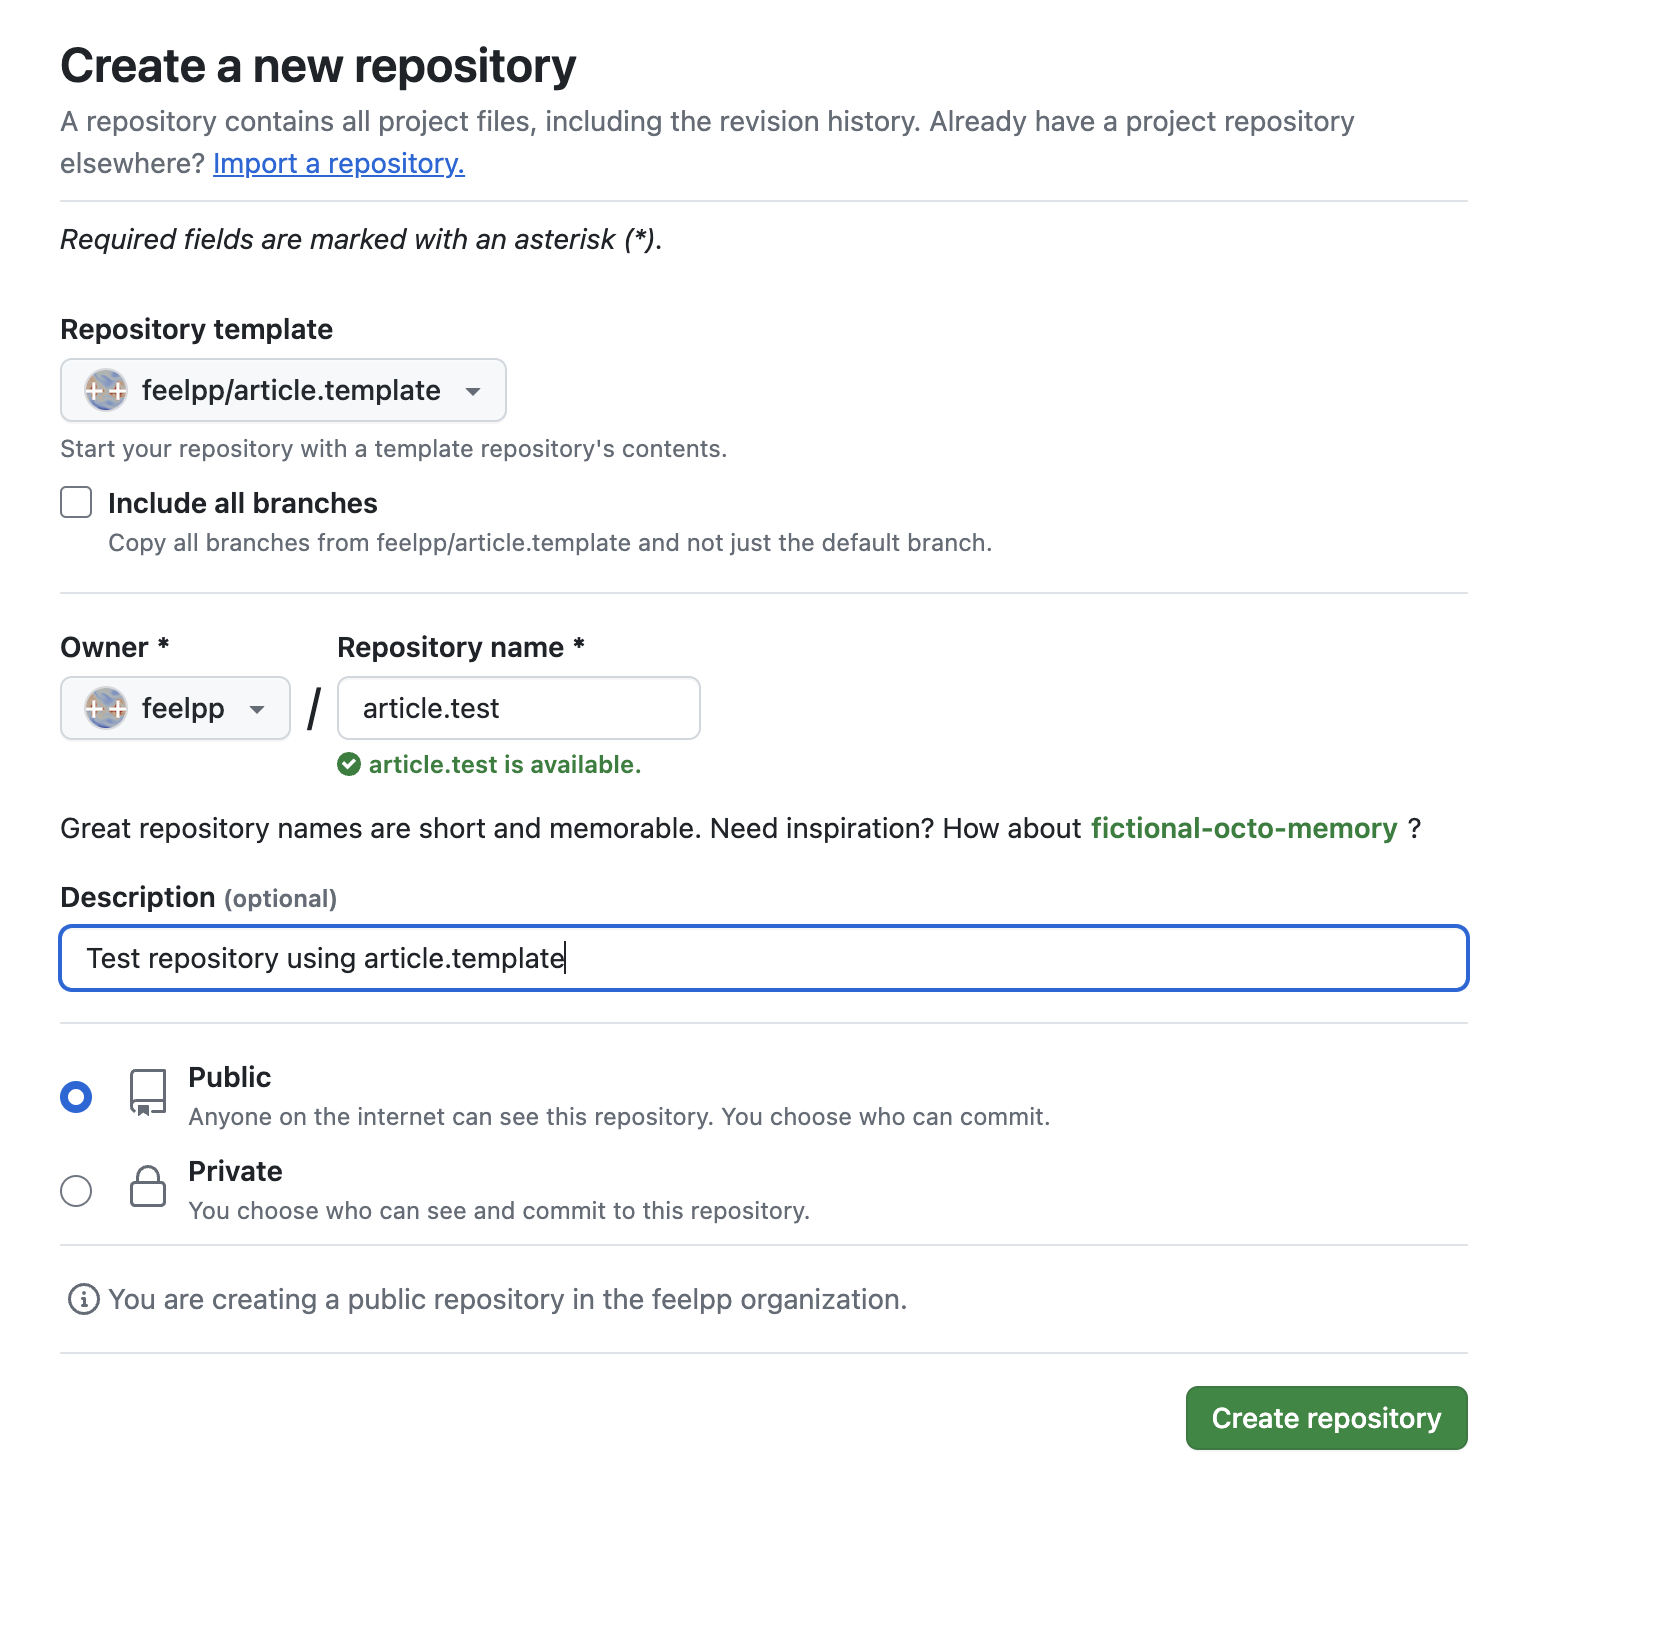
\includegraphics[width=0.8\textwidth]{img-create-repo.png}
\caption{Create a New Repository}
\end{figure}

\subsection{Clone the Repository}
Clone the repository to your local machine.

\begin{minted}[bgcolor=background]{bash}
git clone https://github.com/feelpp/my-repo.git
cd my-repo
\end{minted}

\begin{figure}[h!]
\centering
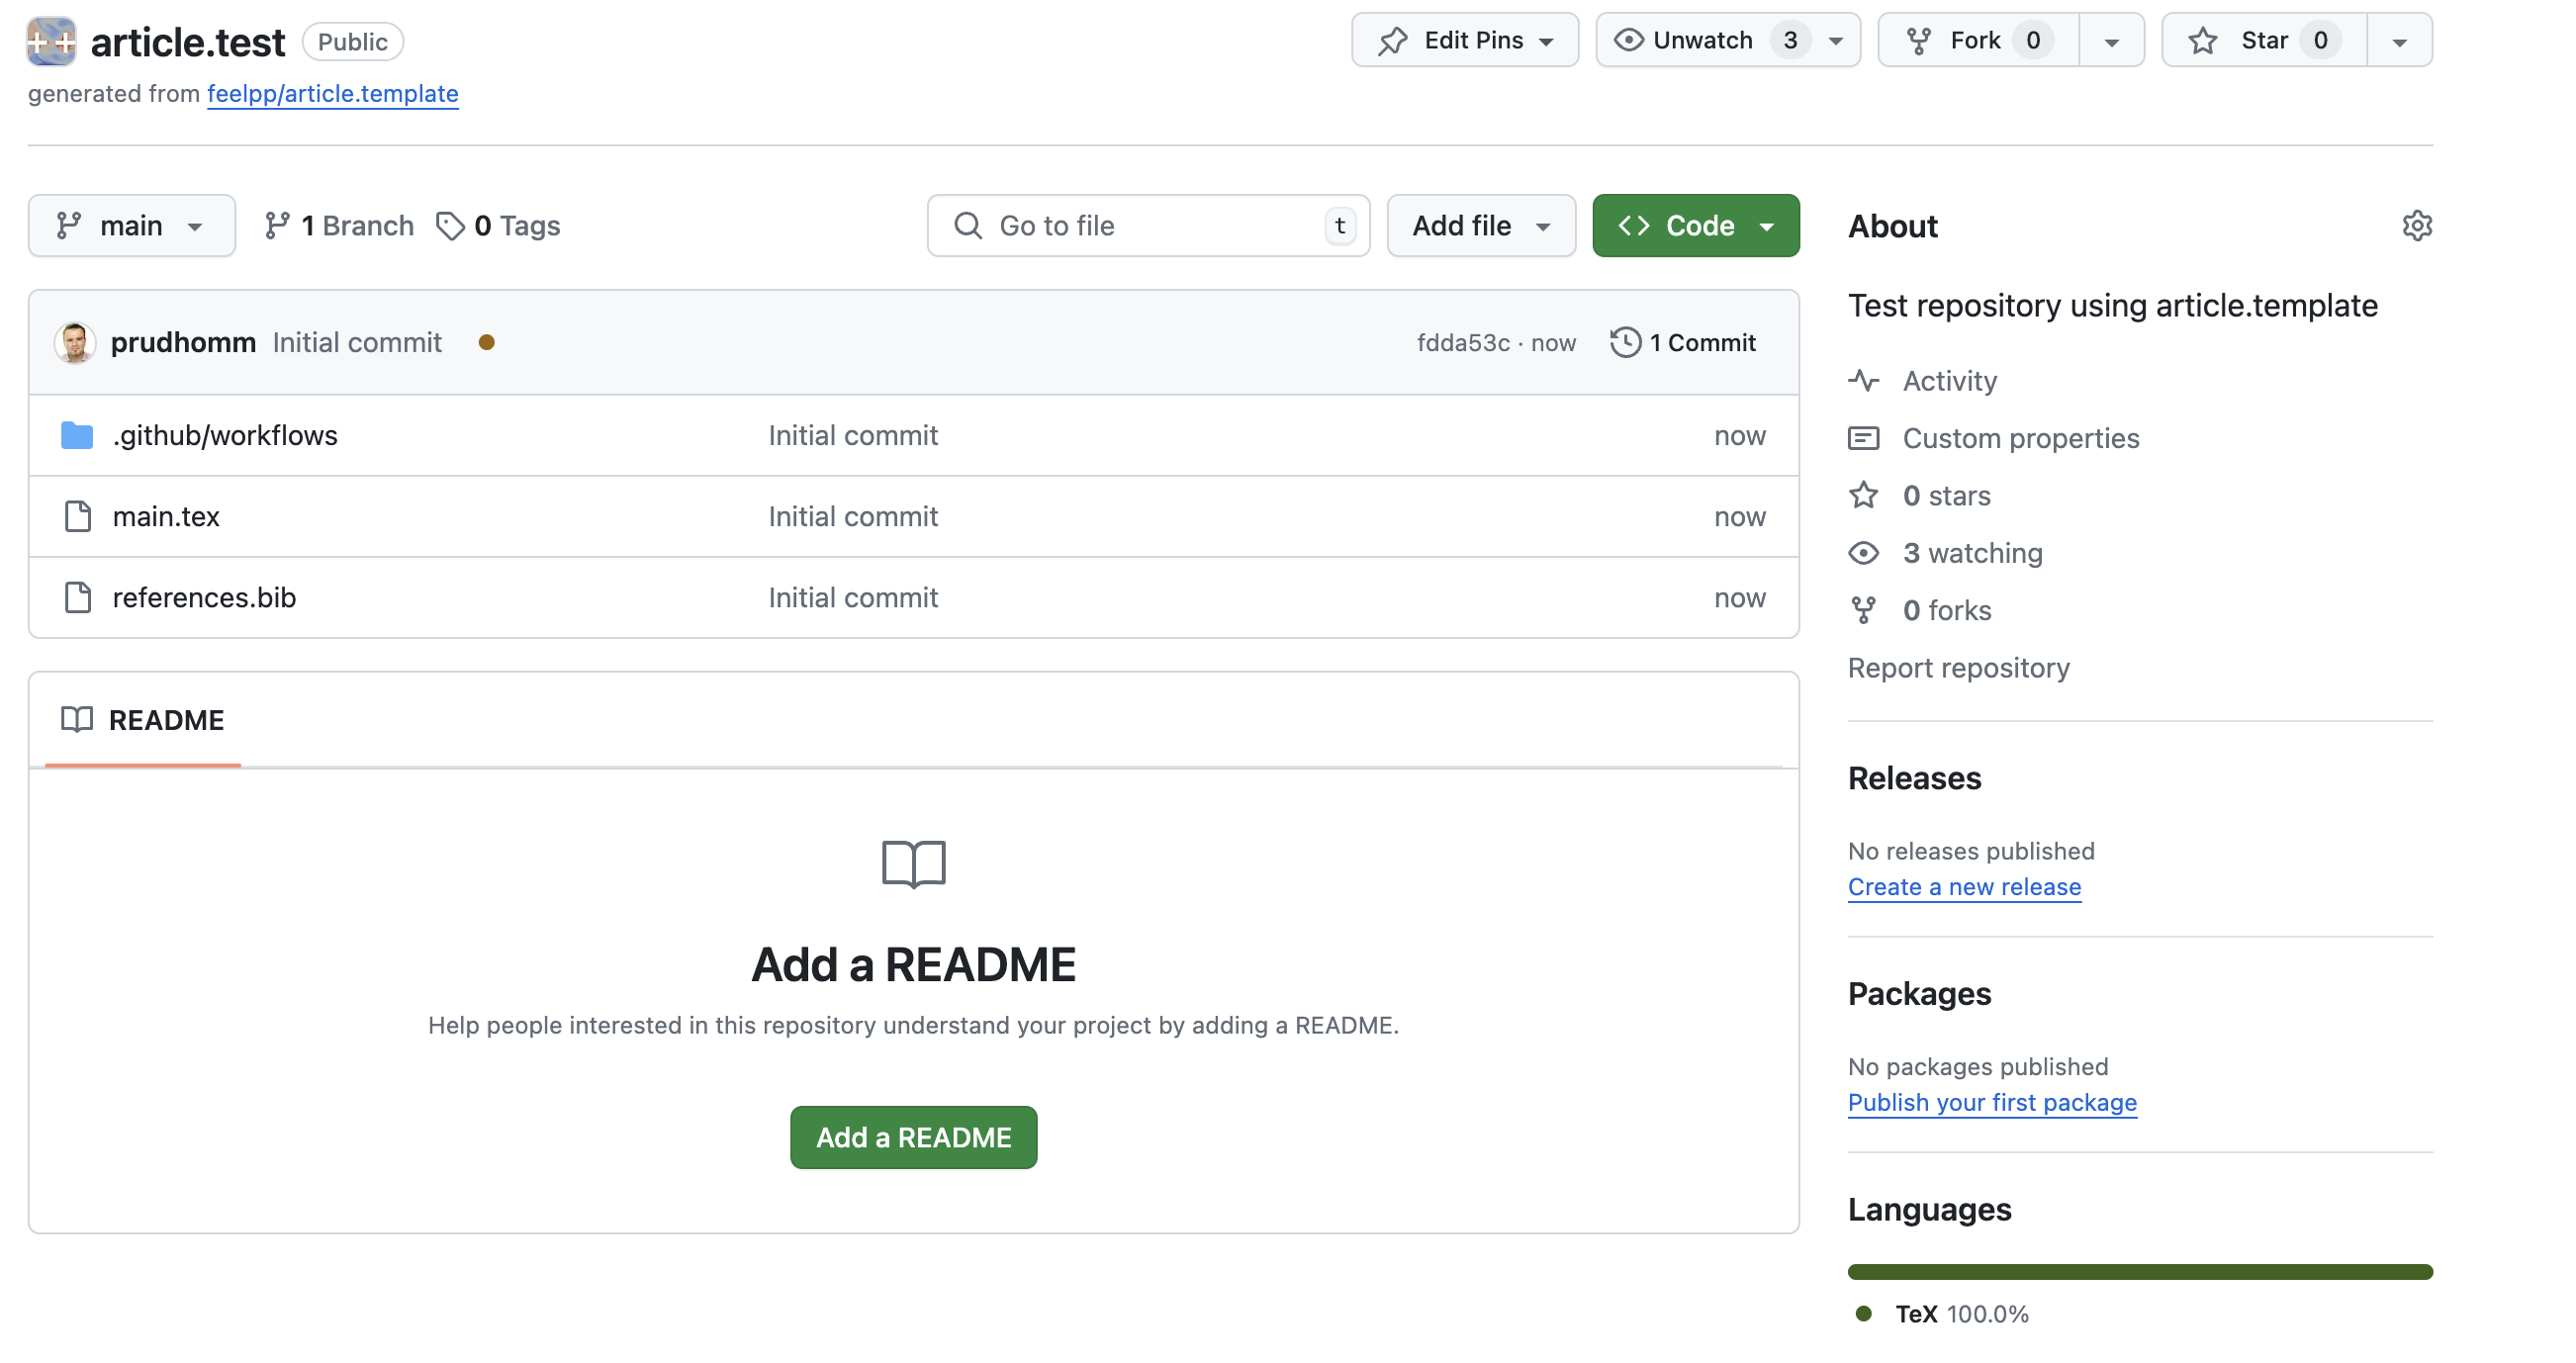
\includegraphics[width=0.8\textwidth]{img-repo-test.png}
\caption{Clone the Repository}
\end{figure}

\subsection{Add Your LaTeX Source Files}
Place your \texttt{.tex} file and image files (\texttt{img-*.pdf}, \texttt{img-*.png}, \texttt{img-*.jpg}) in the repository.

\subsection{Commit and Push Changes}
Commit your changes and push them to the repository.

\begin{minted}[bgcolor=background]{bash}
git add .
git commit -m "Add initial LaTeX document and images"
git push origin main
\end{minted}

The GitHub Action workflow will automatically compile your LaTeX document and upload the resulting PDF as an artifact. You can download the compiled PDF from the Actions tab in your repository.

\section{Overleaf Integration}

\subsection{Sync GitHub Repository with Overleaf}
\begin{enumerate}
    \item In Overleaf, create a new project and select \texttt{Import from GitHub}.
    \item Connect your GitHub account and select the repository you want to sync.
    \item The sync will trigger the workflow and compile your LaTeX document in GitHub.
\end{enumerate}

\subsection{Update References from Zotero}
\begin{enumerate}
    \item Periodically export your references from Zotero to \texttt{references.bib} and push the updated file to your GitHub repository.
    \item Overleaf will automatically sync the changes, ensuring your references are up to date.
\end{enumerate}

\section{Conclusion}
\label{sec:conclusion}

This template provides a comprehensive approach for creating and managing LaTeX articles, integrating modern tools and workflows to enhance productivity and collaboration. 
By leveraging GitHub Actions for automated compilation, Zotero for reference management, and Overleaf for online editing, researchers can streamline the writing process and focus more on content creation. 
The structured setup ensures consistent formatting and efficient handling of images and references, making it suitable for both individual use and collaborative projects.


\bibliographystyle{plainnat}
\bibliography{references}
\end{document}